\documentclass[11pt,a4paper]{article}

% Packages
\usepackage[margin=2.5cm]{geometry}
\usepackage{microtype}
\usepackage{graphicx}
\usepackage{tikz}
\usetikzlibrary{shapes,arrows.meta,positioning,calc,fit,backgrounds,shadows.blur,decorations.pathmorphing,decorations.pathreplacing}
\usepackage{colortbl}
\usepackage{enumitem}
\usepackage{booktabs}
\usepackage{longtable}
\usepackage{hyperref}
\usepackage{xcolor}
\usepackage{fancyhdr}
\usepackage{titlesec}
\usepackage[most]{tcolorbox}
\usepackage{multicol}
\usepackage{amsmath,amssymb}
\usepackage{multirow}
\usepackage{setspace}
\usepackage{fontawesome5}
\usepackage{listings}

% Spacing
\setlength{\parskip}{3pt plus 1pt minus 1pt}
\setlength{\parindent}{0pt}

% Colors
\definecolor{primary}{HTML}{1A5276}
\definecolor{secondary}{HTML}{2E86C1}
\definecolor{accent}{HTML}{E74C3C}
\definecolor{lightbg}{HTML}{EBF5FB}
\definecolor{defbg}{HTML}{FDF2E9}
\definecolor{greenhl}{HTML}{27AE60}
\definecolor{purplehl}{HTML}{8E44AD}
\definecolor{codebg}{HTML}{F4F6F7}

% Hyperref
\hypersetup{colorlinks=true, linkcolor=primary, urlcolor=secondary, citecolor=primary}

% Code listings style
\lstset{
  backgroundcolor=\color{codebg},
  basicstyle=\ttfamily\small,
  keywordstyle=\color{primary}\bfseries,
  stringstyle=\color{greenhl},
  commentstyle=\color{gray},
  breaklines=true,
  frame=l,
  framerule=2pt,
  rulecolor=\color{secondary!40},
  xleftmargin=8pt,
  framexleftmargin=6pt,
  aboveskip=6pt,
  belowskip=6pt,
  showstringspaces=false,
  language=Python
}

% Header/Footer
\pagestyle{fancy}
\fancyhf{}
\fancyhead[L]{\small\textcolor{primary}{\textbf{AI Agents and Agentic AI --- Beginner Foundations}}}
\fancyhead[R]{\small\textcolor{primary}{Lecture Handout}}
\fancyfoot[C]{\small\thepage}
\renewcommand{\headrulewidth}{0.5pt}
\renewcommand{\footrulewidth}{0.3pt}

% Section formatting
\titleformat{\section}{\Large\bfseries\color{primary}}{\thesection}{0.6em}{}[\vspace{2pt}\titlerule]
\titleformat{\subsection}{\large\bfseries\color{secondary}}{\thesubsection}{0.5em}{}
\titleformat{\subsubsection}{\normalsize\bfseries\color{primary}}{\thesubsubsection}{0.5em}{}
\titlespacing*{\section}{0pt}{14pt}{8pt}
\titlespacing*{\subsection}{0pt}{10pt}{5pt}

% Custom boxes
\newtcolorbox{definitionbox}[1][]{
  enhanced, breakable,
  colback=defbg, colframe=orange!60!black,
  colbacktitle=orange!70!black, coltitle=white,
  title={\faIcon{book}~#1}, fonttitle=\bfseries,
  boxrule=0pt, leftrule=4pt, arc=2pt,
  shadow={1mm}{-1mm}{0mm}{black!15},
  top=4pt, bottom=4pt, left=8pt, right=8pt
}
\newtcolorbox{conceptbox}[1][]{
  enhanced, breakable,
  colback=lightbg, colframe=secondary,
  colbacktitle=secondary, coltitle=white,
  title={\faIcon{lightbulb}~#1}, fonttitle=\bfseries,
  boxrule=0pt, leftrule=4pt, arc=2pt,
  shadow={1mm}{-1mm}{0mm}{black!15},
  top=4pt, bottom=4pt, left=8pt, right=8pt
}
\newtcolorbox{alertbox}[1][]{
  enhanced, breakable,
  colback=red!4, colframe=accent,
  colbacktitle=accent, coltitle=white,
  title={\faIcon{exclamation-triangle}~#1}, fonttitle=\bfseries,
  boxrule=0pt, leftrule=4pt, arc=2pt,
  shadow={1mm}{-1mm}{0mm}{black!12},
  top=3pt, bottom=3pt, left=8pt, right=8pt
}
\newtcolorbox{examplebox}[1][]{
  enhanced, breakable,
  colback=green!4, colframe=greenhl,
  colbacktitle=greenhl, coltitle=white,
  title={\faIcon{code}~#1}, fonttitle=\bfseries,
  boxrule=0pt, leftrule=4pt, arc=2pt,
  shadow={1mm}{-1mm}{0mm}{black!12},
  top=3pt, bottom=3pt, left=8pt, right=8pt
}

\begin{document}

% Title
\begin{center}
\vspace*{0.5cm}
{\Huge\bfseries\textcolor{primary}{AI Agents and Agentic AI}}\\[8pt]
{\Huge\bfseries\textcolor{primary}{Comprehensive Beginner Handout}}\\[16pt]
{\color{secondary}\rule{0.68\textwidth}{1.5pt}}\\[14pt]
{\Large\textsc{Data Science Course --- BSIT Program}}\\[8pt]
{\large\textcolor{gray!70!black}{Concepts $\bullet$ Workflows $\bullet$ Tools $\bullet$ GitHub Copilot $\bullet$ Responsible Use}}
\vspace{0.3cm}
\end{center}

\tableofcontents
\newpage

%=============================================================
\section{Introduction to AI Agents}
%=============================================================

\begin{definitionbox}[AI Agent]
An AI agent is a system that can \textbf{understand a goal, decide what to do next, use available tools, observe results, and continue until the task is finished or stopped}. It is more than a simple chatbot because it can work through \textbf{multiple steps} instead of only giving one direct answer.
\end{definitionbox}

\begin{definitionbox}[Agentic AI]
Agentic AI refers to AI systems that behave in a more goal-directed and action-oriented way. These systems can \textbf{plan, reason, use tools, keep track of state, and take follow-up actions} with limited human intervention.
\end{definitionbox}

\begin{conceptbox}[Simple Meaning]
If a system only answers one question at a time, it behaves like a basic assistant. If it can break a task into steps, search for information, write files, call tools, and revise its work, it is acting in a more \textbf{agentic} way.
\end{conceptbox}

\subsection{Where AI Agents Fit in AI}

\begin{center}
\begin{tikzpicture}[scale=1]
  \fill[black!8] (0.08,-0.08) circle (4.7cm);
  \fill[blue!6] (0,0) circle (4.7cm);
  \draw[thick, primary, line width=1.5pt] (0,0) circle (4.7cm);
  \node[font=\bfseries\large, primary] at (0,4.0) {\faIcon{robot}~Artificial Intelligence};
  \node[font=\scriptsize, primary!70, align=center] at (3.3,-3.25) {Search, planning,\\recommendation,\\automation};

  \fill[orange!8] (0,-0.4) circle (3.0cm);
  \draw[thick, orange!70!black, line width=1.2pt] (0,-0.4) circle (3.0cm);
  \node[font=\bfseries, orange!70!black] at (0,2.1) {\faIcon{brain}~Machine Learning};
  \node[font=\scriptsize, orange!50!black, align=center] at (-2.2,0.25) {Classification,\\prediction,\\pattern learning};

  \fill[green!8] (0,-0.7) circle (1.7cm);
  \draw[thick, greenhl!70!black, line width=1.2pt] (0,-0.7) circle (1.7cm);
  \node[font=\bfseries\small, greenhl!70!black, align=center] at (0,-0.7) {\faIcon{project-diagram}\\AI Agents\\and Agentic AI};
\end{tikzpicture}
\end{center}

\begin{itemize}[leftmargin=*]
  \item \textbf{Artificial Intelligence} is the broad field of making systems act intelligently.
  \item \textbf{Machine Learning} is a subset that learns from data.
  \item \textbf{AI Agents} are intelligent systems that pursue goals through steps, decisions, and actions.
\end{itemize}

\subsection{Why AI Agents Matter}

\begin{itemize}[leftmargin=*]
  \item They help automate repetitive and multi-step work.
  \item They can combine reasoning with tools such as search, files, APIs, and databases.
  \item They are useful in education, business, software engineering, data analysis, and customer support.
  \item They represent a practical shift from simple AI responses to task completion.
\end{itemize}

%=============================================================
\section{AI Agent vs Chatbot vs Traditional Automation}
%=============================================================

\begin{center}
\begin{tabular}{@{}p{3.2cm}p{3.6cm}p{3.6cm}p{3.2cm}@{}}
\toprule
\textbf{System} & \textbf{Main Behavior} & \textbf{Strength} & \textbf{Limitation} \\
\midrule
Basic chatbot & Answers direct questions & Easy to use & Usually limited to one-turn responses \\
Traditional automation & Follows fixed rules or scripts & Reliable for repeated tasks & Cannot adapt well to new situations \\
AI agent & Plans, acts, checks results, and continues & More flexible and capable & Needs guardrails and monitoring \\
\bottomrule
\end{tabular}
\end{center}

\begin{conceptbox}[Key Difference]
A chatbot mainly \textbf{responds}. An AI agent can \textbf{respond, decide, act, observe, and continue working}.
\end{conceptbox}

%=============================================================
\section{Core Components of an AI Agent}
%=============================================================

\rowcolors{2}{white}{defbg}
\begin{longtable}{@{}p{3.6cm}p{9.9cm}@{}}
\toprule
\rowcolor{primary!15}
\textbf{Component} & \textbf{Purpose} \\
\midrule
\endhead
Goal or instruction & Defines what the agent is trying to achieve \\
\addlinespace
Model or reasoning engine & Interprets input and decides what to do next \\
\addlinespace
Memory or state & Stores conversation history, facts, or intermediate work \\
\addlinespace
Tools & Allow the agent to search, calculate, code, call APIs, or edit files \\
\addlinespace
Environment & The world or system the agent interacts with \\
\addlinespace
Guardrails & Safety rules, permissions, and limits on what the agent can do \\
\addlinespace
Feedback loop & Lets the agent check progress and revise if needed \\
\bottomrule
\end{longtable}

\subsection{Easy Interpretation of the Components}

\begin{itemize}[leftmargin=*]
  \item The \textbf{goal} tells the agent what success looks like.
  \item The \textbf{model} provides reasoning and generation ability.
  \item \textbf{Memory} prevents the agent from starting from zero every time.
  \item \textbf{Tools} let the agent do real work beyond text generation.
  \item \textbf{Guardrails} reduce misuse, errors, and unsafe actions.
\end{itemize}

%=============================================================
\section{The Agent Loop: Sense, Think, Act, Observe}
%=============================================================

\begin{center}
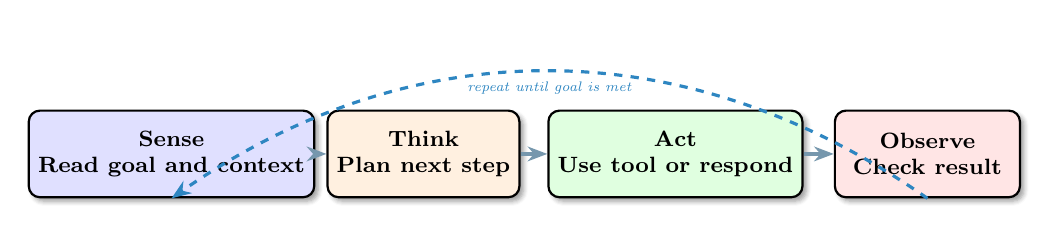
\begin{tikzpicture}[
  step/.style={rectangle, draw, thick, fill=#1, minimum width=2.35cm, minimum height=1.1cm, align=center, font=\footnotesize\bfseries, rounded corners=4pt,
    blur shadow={shadow blur steps=5, shadow xshift=0.5mm, shadow yshift=-0.5mm}},
  arr/.style={-{Stealth[length=2.5mm]}, very thick, primary!60, line width=1.15pt}
]
  \node[step=blue!12] (s1) at (0,0) {Sense\\Read goal and context};
  \node[step=orange!12] (s2) at (3.2,0) {Think\\Plan next step};
  \node[step=green!12] (s3) at (6.4,0) {Act\\Use tool or respond};
  \node[step=red!10] (s4) at (9.6,0) {Observe\\Check result};

  \draw[arr] (s1) -- (s2);
  \draw[arr] (s2) -- (s3);
  \draw[arr] (s3) -- (s4);
  \draw[arr, dashed, secondary] (s4.south) to[bend right=35] node[below, font=\tiny\itshape, secondary] {repeat until goal is met} (s1.south);
\end{tikzpicture}
\end{center}

\begin{definitionbox}[Agent Loop]
Most AI agents operate through a repeating cycle:
\begin{itemize}[leftmargin=*]
  \item \textbf{Sense:} Understand the prompt, files, history, or environment.
  \item \textbf{Think:} Decide what should happen next.
  \item \textbf{Act:} Use a tool, generate content, or modify something.
  \item \textbf{Observe:} Review the result and decide whether to continue.
\end{itemize}
\end{definitionbox}

%=============================================================
\section{Memory, Tools, and Planning}
%=============================================================

\subsection{Memory}

\begin{definitionbox}[Memory in Agents]
Memory allows an agent to store useful information from previous steps, such as user preferences, earlier outputs, temporary notes, or task history.
\end{definitionbox}

\begin{itemize}[leftmargin=*]
  \item \textbf{Short-term memory:} Current conversation or current task state.
  \item \textbf{Long-term memory:} Stored preferences, facts, or reusable knowledge.
\end{itemize}

\subsection{Tools}

\begin{definitionbox}[Tool Use]
Tool use means the agent can call external capabilities rather than only generate text. Tools may include web search, file editing, database access, Python execution, calculators, or application commands.
\end{definitionbox}

\begin{examplebox}[Simple Example]
If a user asks, \textit{``Create a report from this CSV file,''} a basic chatbot may only describe the steps. An agentic system can open the file, analyze the data, generate the report, and save the result.
\end{examplebox}

\subsection{Planning}

\begin{conceptbox}[Planning]
Planning means breaking one large task into smaller steps. For example, instead of trying to solve everything at once, an agent can first inspect the data, then clean it, then analyze it, then summarize the results.
\end{conceptbox}

%=============================================================
\section{Types of AI Agents}
%=============================================================

\rowcolors{2}{white}{defbg}
\begin{longtable}{@{}p{3.4cm}p{3.5cm}p{5.9cm}@{}}
\toprule
\rowcolor{primary!15}
\textbf{Type} & \textbf{Main Idea} & \textbf{Example} \\
\midrule
\endhead
Single agent & One agent handles the whole task & A coding assistant that completes one workflow \\
\addlinespace
Multi-agent system & Several agents share responsibilities & Planner agent plus researcher agent plus reviewer agent \\
\addlinespace
Reactive agent & Responds based on current situation & A support bot answering FAQ prompts \\
\addlinespace
Goal-based agent & Chooses steps to reach a target & An assistant that prepares a complete project file \\
\addlinespace
Tool-using agent & Calls external tools to act & A data agent that runs SQL or Python \\
\bottomrule
\end{longtable}

\subsection{Single-Agent vs Multi-Agent}

\begin{center}
\begin{tabular}{@{}p{6.3cm}p{6.3cm}@{}}
\toprule
\textbf{Single-Agent System} & \textbf{Multi-Agent System} \\
\midrule
Simpler to build and manage & More modular and specialized \\
Fewer coordination problems & Better for dividing complex tasks \\
Easier to monitor & More overhead and more communication complexity \\
Useful for focused tasks & Useful for large workflows or teams of functions \\
\bottomrule
\end{tabular}
\end{center}

%=============================================================
\section{Large Language Models and AI Agents}
%=============================================================

\begin{definitionbox}[LLM as the Reasoning Core]
Modern AI agents are often built around Large Language Models (LLMs). The LLM helps the agent understand instructions, generate explanations, choose next steps, and interact in natural language.
\end{definitionbox}

\begin{conceptbox}[Important Distinction]
An LLM by itself is not always a full agent. It becomes part of an agentic system when it is connected to \textbf{goals, memory, tools, and feedback loops}.
\end{conceptbox}

\begin{itemize}[leftmargin=*]
  \item An LLM helps with language understanding and generation.
  \item Tools help the system take external actions.
  \item Memory helps it keep track of what has happened.
  \item Planning helps it complete multi-step tasks.
\end{itemize}

%=============================================================
\section{Key Beginner Terms}
%=============================================================

\rowcolors{2}{white}{defbg}
\begin{longtable}{@{}p{3.4cm}p{10cm}@{}}
\toprule
\rowcolor{primary!15}
\textbf{Term} & \textbf{Meaning} \\
\midrule
\endhead
Prompt & The instruction given to the system \\
\addlinespace
State & The current situation or memory of the task \\
\addlinespace
Action & Something the agent does, such as calling a tool or writing text \\
\addlinespace
Observation & The result of an action \\
\addlinespace
Tool call & A request sent to a calculator, file system, API, or application \\
\addlinespace
Planning & Dividing a task into steps \\
\addlinespace
Reasoning & Deciding what action makes sense next \\
\addlinespace
Guardrail & A control that limits unsafe or incorrect behavior \\
\addlinespace
Autonomy & The amount of work the agent can do without direct human guidance \\
\addlinespace
Human in the loop & A human reviewer approves or checks important steps \\
\bottomrule
\end{longtable}

%=============================================================
\section{GitHub Copilot as an Example of Agentic AI}
%=============================================================

\begin{definitionbox}[GitHub Copilot]
GitHub Copilot is an AI coding assistant that helps users write, explain, edit, and navigate code. In modern development environments, it is not limited to autocomplete. It can also support chat-based help, multi-file edits, and more agentic workflows.
\end{definitionbox}

\subsection{Why Copilot Matters in Data Science}

\begin{itemize}[leftmargin=*]
  \item It can help write Python, SQL, R, and notebook code.
  \item It can explain libraries, functions, and error messages.
  \item It can help generate visualizations, summaries, and documentation.
  \item It can support experimentation, debugging, and project organization.
\end{itemize}

\subsection{Common Copilot Experiences}

\begin{itemize}[leftmargin=*]
  \item \textbf{Inline code completion:} Suggests code while you type.
  \item \textbf{Chat assistance:} Answers questions and explains code or concepts.
  \item \textbf{Editing assistance:} Applies requested changes to code or text.
  \item \textbf{Agentic workflow support:} Can inspect a workspace, make a series of edits, and validate changes.
\end{itemize}

\subsection{GitHub Copilot Modes}

\begin{conceptbox}[Mode Names Can Vary by Version or Editor]
GitHub Copilot features change over time. In VS Code and similar environments, the most important beginner-level distinction is between \textbf{asking}, \textbf{editing}, and \textbf{agent-like task execution}. The names and exact buttons may vary across versions.
\end{conceptbox}

\rowcolors{2}{white}{defbg}
\begin{longtable}{@{}p{2.7cm}p{3.8cm}p{5.9cm}@{}}
\toprule
\rowcolor{primary!15}
\textbf{Mode} & \textbf{What It Does} & \textbf{Typical Use} \\
\midrule
\endhead
Ask mode & Answers questions, explains code, suggests approaches & Learn concepts, debug errors, understand algorithms, ask for examples \\
\addlinespace
Edit mode & Applies requested changes to code or text & Refactor functions, update notebooks, fix formatting, rewrite blocks \\
\addlinespace
Agent mode & Works through a multi-step task using repo context and tools & Search files, update several places, run validations, complete coding tasks \\
\bottomrule
\end{longtable}

\subsection{How Students Should Use Copilot}

\begin{itemize}[leftmargin=*]
  \item Use \textbf{Ask mode} to understand topics before copying code.
  \item Use \textbf{Edit mode} when you already know what you want changed.
  \item Use \textbf{Agent mode} for larger tasks that involve multiple steps or files.
  \item Always test and review outputs, especially for assignments or data analysis.
\end{itemize}

\begin{alertbox}[Important Academic Note]
Copilot can speed up learning, but students should not rely on it blindly. The user is still responsible for correctness, originality, and understanding the submitted work.
\end{alertbox}

%=============================================================
\section{Applications of AI Agents in Data Science}
%=============================================================

\begin{itemize}[leftmargin=*]
  \item \textbf{Data collection assistance:} gathering information from files, APIs, or structured sources.
  \item \textbf{Data cleaning support:} suggesting preprocessing steps and detecting common issues.
  \item \textbf{Exploratory data analysis:} generating charts, summaries, and descriptive interpretations.
  \item \textbf{Modeling assistance:} recommending algorithms, hyperparameters, and evaluation approaches.
  \item \textbf{Documentation and reporting:} summarizing findings into readable reports.
  \item \textbf{Notebook guidance:} helping explain code cells, functions, and outputs.
\end{itemize}

\subsection{BSIT-Relevant Examples}

\begin{examplebox}[Examples for BSIT Students]
\begin{itemize}[leftmargin=*]
  \item An agent that explains Python code in a Jupyter notebook.
  \item An agent that cleans CSV data and produces a short summary.
  \item An agent that drafts documentation for a class project.
  \item An agent that helps compare machine learning models and metrics.
  \item A campus support bot that answers student questions using official information.
\end{itemize}
\end{examplebox}

%=============================================================
\section{Benefits of AI Agents}
%=============================================================

\begin{itemize}[leftmargin=*]
  \item Reduce repetitive work.
  \item Combine information from many tools and sources.
  \item Support faster workflows and decision-making.
  \item Provide more interactive and personalized assistance.
  \item Help users move from ideas to results more quickly.
\end{itemize}

%=============================================================
\section{Risks, Limitations, and Challenges}
%=============================================================

\rowcolors{2}{white}{defbg}
\begin{longtable}{@{}p{3.1cm}p{4.1cm}p{6.1cm}@{}}
\toprule
\rowcolor{primary!15}
\textbf{Risk} & \textbf{Meaning} & \textbf{Possible Response} \\
\midrule
\endhead
Hallucination & The system produces false or unsupported information & Verify important outputs and use trusted data \\
\addlinespace
Unsafe tool use & A tool call may change or expose data incorrectly & Add permissions and approval checkpoints \\
\addlinespace
Prompt injection & Malicious instructions try to manipulate the system & Validate inputs and restrict tool access \\
\addlinespace
Privacy risk & Sensitive data may be revealed or misused & Avoid unnecessary sharing and protect confidential data \\
\addlinespace
Over-automation & Users trust the system too much & Keep humans involved in critical decisions \\
\bottomrule
\end{longtable}

\begin{definitionbox}[Hallucination]
Hallucination means the AI gives an answer that sounds correct but is actually false, incomplete, or invented.
\end{definitionbox}

\begin{definitionbox}[Prompt Injection]
Prompt injection is an attack or manipulation attempt where the input tries to override the intended rules of the system and force it into unsafe or incorrect behavior.
\end{definitionbox}

%=============================================================
\section{Best Practices for Building or Using Agents}
%=============================================================

\begin{itemize}[leftmargin=*]
  \item Start with a narrow and clear task.
  \item Limit what tools the agent can use.
  \item Keep logs of important actions.
  \item Validate important outputs before using them.
  \item Use human approval for high-impact steps.
  \item Measure accuracy, latency, cost, and safety.
  \item Test with normal inputs and edge cases.
  \item Explain to users what the agent can and cannot do.
\end{itemize}

\begin{conceptbox}[Practical Rule]
The best beginner agent systems are not the most autonomous ones. They are the ones that are \textbf{clear, narrow, testable, and safe}.
\end{conceptbox}

%=============================================================
\section{Mini Case Study for BSIT Data Science}
%=============================================================

\begin{definitionbox}[Scenario]
A BSIT Data Science class wants an assistant that can help students understand assignments, explain dataset columns, generate starter analysis code, and summarize notebook results.
\end{definitionbox}

\textbf{Possible workflow:}
\begin{enumerate}[leftmargin=*]
  \item The student asks a question about a dataset or notebook.
  \item The agent reads the prompt and relevant files.
  \item It plans what information to inspect first.
  \item It generates an explanation or starter code.
  \item It checks whether the result matches the student's requested level.
  \item The student reviews and tests the answer before using it.
\end{enumerate}

\begin{alertbox}[Responsible Use in Education]
An educational agent should support learning, not replace understanding. Students still need to read, test, and explain their own work.
\end{alertbox}

%=============================================================
\section{A Small Pseudocode Example}
%=============================================================

\begin{lstlisting}
goal = "Summarize this dataset and suggest first analysis steps"

context = read_file("students.csv")
plan = agent.plan(goal, context)
result = agent.use_tools(plan)
checked = agent.review(result)

print(checked)
\end{lstlisting}

\begin{conceptbox}[What This Shows]
The agent receives a goal, reads context, creates a plan, uses tools, reviews the result, and then returns an answer. This is the basic logic behind many modern agent systems.
\end{conceptbox}

%=============================================================
\section{Summary}
%=============================================================

\begin{itemize}[leftmargin=*]
  \item AI agents are systems that pursue goals through repeated cycles of understanding, acting, and checking.
  \item Agentic AI combines reasoning, planning, memory, and tool use.
  \item Agents differ from simple chatbots because they can complete multi-step tasks.
  \item Modern agents often use LLMs, but LLMs alone are not full agents.
  \item GitHub Copilot is a useful example of agentic assistance in coding and Data Science workflows.
  \item Copilot is commonly understood through three practical modes: Ask, Edit, and Agent.
  \item AI agents can be powerful, but they require validation, guardrails, and responsible use.
\end{itemize}

%=============================================================
\section{Review Questions}
%=============================================================

\begin{enumerate}[leftmargin=*]
  \item What is the difference between an AI agent and a basic chatbot?
  \item What does the term agentic AI mean?
  \item Why are memory and tools important in an agent system?
  \item What happens in the sense-think-act-observe loop?
  \item How does a single-agent system differ from a multi-agent system?
  \item Why is an LLM not always a complete agent by itself?
  \item What are the main purposes of GitHub Copilot Ask mode, Edit mode, and Agent mode?
  \item What are some useful applications of AI agents in Data Science?
  \item What is hallucination, and why is it dangerous?
  \item Why should human review remain part of agent-based systems?
\end{enumerate}

\end{document}